\documentclass[12pt]{article}
\usepackage[utf8]{inputenc}
\usepackage{amsmath}
\usepackage{amssymb}
\usepackage{graphicx}
\usepackage{hyperref}
\usepackage{geometry}
\usepackage{booktabs}
\usepackage{algorithm}
\usepackage{algpseudocode}
\usepackage{tikz}
\usepackage{pgfplots}

% Increase the bottom margin
\geometry{bottom=1in, left=1in, right=1in, top=1in} % Adjust the value as needed

\title{CS312 Project 5 Report}
\author{}
\date{}

\begin{document}

\maketitle

\tableofcontents

\section{Complexity Analysis}

\subsection{Greedy}
\begin{algorithm}[H]
    \caption{\textsc{Greedy\_TSP}}
    \begin{algorithmic}[1]
        \State \textbf{Input:} graph
        \State \textbf{Initialize:} \texttt{bestPath} $\gets$ \texttt{None}, \texttt{bestCost} $\gets \infty$
        \For{\texttt{eachNode} in graph.nodes} \Comment{runs $n$ times}
            \State \texttt{currentNode} $\gets$ \texttt{eachNode}
            \State \texttt{visitedNodes} $\gets$ empty set
            \State Add \texttt{currentNode} to \texttt{visitedNodes}
            \State \texttt{path} $\gets$ [\texttt{currentNode}]
            \State \texttt{currentCost} $\gets 0$
            \While{there are unvisited nodes} \Comment{runs $n$ times}
                \State Find the nearest unvisited neighbor of \texttt{currentNode}
                \State Add the neighbor to \texttt{visitedNodes}
                \State Append the neighbor to \texttt{path}
                \State Update \texttt{currentCost} with the cost to the neighbor
                \State \texttt{currentNode} $\gets$ neighbor
            \EndWhile
            \If{\texttt{currentCost} $<$ \texttt{bestCost}}
                \State \texttt{bestCost} $\gets$ \texttt{currentCost}
                \State \texttt{bestPath} $\gets$ \texttt{path}
            \EndIf
        \EndFor
        \State \Return \texttt{bestPath} and \texttt{bestCost}
    \end{algorithmic}
\end{algorithm}

My implementation of the greedy TSP algorithm uses nested loops which each iterate
over the n nodes in the graph. The outer loop runs $n$ times, and the inner loop
runs $n$ times as well, leading to a time complexity of $O(n^2)$. The space complexity
scales only with the number of nodes; a best path and a current path are stored, each of
length $n$ or less. All other storage is constant. Thus, the space complexity is $O(n)$.

\newpage

\subsection{DFS}
\begin{algorithm}[H]
    \caption{\textsc{DFS\_TSP}}
    \begin{algorithmic}[1]
        \State \textbf{Input:} graph
        \State \textbf{Initialize:} \texttt{bestPath} $\gets$ \texttt{None}, \texttt{bestCost} $\gets \infty$
        \State \texttt{visitedNodes} $\gets$ empty set
        \State \texttt{path} $\gets$ empty list
        \State \texttt{currentCost} $\gets 0$
        \State Call \textsc{DFS}(graph, visitedNodes, path, currentCost) \Comment{$O(n!)$}
    \end{algorithmic}
\end{algorithm}


\begin{algorithm}[H]
    \caption{\textsc{DFS}}
    \begin{algorithmic}[1]
        \State \textbf{Input:} graph, path
        \If{all nodes are in path}
            \If{there is an edge back to the start node}
                \State \texttt{cost} $\gets$ compute the cost of \texttt{path}
                \If{\texttt{cost} $<$ \texttt{bestCost}}
                    \State \texttt{bestCost} $\gets$ \texttt{cost}
                    \State \texttt{bestPath} $\gets$ \texttt{path}
                \EndIf
            \EndIf
            \State \Return
        \EndIf
        \For{\texttt{neighbor} in neighbors of the last node in \texttt{path}} \Comment{runs $n$ times}
            \If{\texttt{neighbor} is not visited and edge exists}
                \State Call \textsc{DFS}(graph, path + [\texttt{neighbor}]) \Comment{runs max $n$ - depth times}
            \EndIf
        \EndFor
    \end{algorithmic}
\end{algorithm}

My implementation of the DFS TSP algorithm uses a recursive function to
explore all possible paths. The outer function runs $n$ times, and the inner
function runs at most $n$ - recursion depth times. This leads to a time complexity of
$O(n!)$, as shown by the following equation:
\[
n \times (n-1) \times (n-2) \times \dots \times 1 = n!
\]
The space complexity is $O(n)$, as the only non-constant space used is the call stack, path,
and visited nodes, which are all $O(n)$.

\newpage

\subsection{Branch-and-Bound}
\begin{algorithm}[H]
    \caption{\textsc{Branch-and-Bound}}
    \begin{algorithmic}[1]
        \State \textbf{Input:} graph
        \State \texttt{bestScore, bestPath} $\gets$ \textsc{greedy\_tsp}(graph) \Comment{$O(n^2)$}
        \State \texttt{edgesCopy} $\gets$ copy of edges with diagonal set to $\infty$
        \State \texttt{edgesCopy}, \texttt{lowerBound} $\gets$ \textsc{Reduce\_Matrix}(\texttt{edgesCopy})
        \State \textsc{BB\_Helper}([0], \texttt{edgesCopy}, \texttt{lowerBound}) \Comment{$O(n!)$}
        \State \Return \texttt{bestScore} and \texttt{bestPath}
    \end{algorithmic}
\end{algorithm}

\begin{algorithm}[H]
    \caption{\textsc{BB\_Helper}}
    \begin{algorithmic}[1]
        \If{\texttt{len(tour)} $=$ \texttt{len(reducedEdges)} \textbf{and} there is return edge}
            \State \texttt{cost} $\gets$ \textsc{Score\_Tour}(\texttt{tour}, edges)
            \If{\texttt{cost} $<$ \texttt{bestScore}}
                \State \texttt{bestScore} $\gets$ \texttt{cost}, \texttt{bestTour} $\gets$ \texttt{tour}
            \EndIf
            \State \Return
        \EndIf
        \For{\texttt{i} in range of \texttt{len(reducedEdges)}} \Comment{runs $n$ times}
            \If{\texttt{reducedEdges[tour[-1]][i]} $=$ $\infty$ \textbf{or} \texttt{i} in \texttt{tour}}
                \State \textbf{continue}
            \EndIf
            \State \texttt{newMatrix}, \texttt{pathCost} $\gets$ \textsc{Update\_Matrix}(\texttt{reducedEdges}, \texttt{tour[-1]}, \texttt{i})
            \State \texttt{newLowerBound} $\gets$ \texttt{lowerBound} $+$ \texttt{pathCost}
            \If{\texttt{newLowerBound} $<$ \texttt{bestScore}} \Comment{called at most $n$ - depth times}
                \State \textsc{BB\_Helper}(\texttt{tour} $+$ [\texttt{i}], \texttt{newMatrix}, \texttt{newLowerBound}) 
            \EndIf
        \EndFor
    \end{algorithmic}
\end{algorithm}

My implementation of the branch-and-bound algorithm uses a recursive function
to explore all possible paths. A baseline value is calculated using the greedy
algorithm, which runs in $O(n^2)$ time. The outer function runs $n$ times, and the inner
function runs at most $n$ - recursion depth times, leading to that many potential child nodes.
The inner functions run in $O(n^2)$ time,
as shown below. This leads to a maximum time complexity of
$O(n! \times n^2) = O(n!)$. However, branches are pruned when the lower bound
is greater than the best score, leading to better possible time complexity, down to 
$O(n^2)$ in the best case, the best path is found in the first iteration. The max space
complexity is also $O(n!)$, because the $n \times n $ reduced matrix is stored at
 all steps in the call stack.

\newpage

\begin{algorithm}
    \caption{\textsc{Reduce\_Matrix}}
    \begin{algorithmic}[1]
        \State \textbf{Input:} graph
        \State \texttt{matrix} $\gets$ copy of graph.edges
        \State \texttt{rowReduction} $\gets$ 0
        \For{row \texttt{i} in \texttt{matrix.length}} \Comment{runs $n$ times}
            \State \texttt{minVal} $\gets$ min value in row \texttt{i}
            \If{\texttt{minVal} $>$ 0}
                \State \texttt{rowReduction} $+$= \texttt{minVal}
                \State Subtract \texttt{minVal} from each element in row \Comment{$O(n)$}
            \EndIf
        \EndFor
        \For{column \texttt{j} in \texttt{matrix[0].length}} \Comment{runs $n$ times}
            \State \texttt{minVal} $\gets$ min value in column \texttt{j}
            \If{\texttt{minVal} $>$ 0}
                \State \texttt{rowReduction} $+$= \texttt{minVal}
                \State Subtract \texttt{minVal} from each element in column \Comment{$O(n)$}
            \EndIf
        \EndFor
        \State \Return \texttt{matrix}, \texttt{rowReduction}
    \end{algorithmic}
\end{algorithm}

\begin{algorithm}
    \caption{\textsc{Update\_Matrix}}
    \begin{algorithmic}[1]
        \State \textbf{Input:} graph, row, column
        \State \texttt{matrix} $\gets$ copy of graph
        \State \texttt{pathCost} $\gets$ matrix[row][column]
        \For{\texttt{i} in range of matrix.length} \Comment{runs $n$ times}
            \State matrix[\texttt{i}][column] $\gets$ $\infty$
            \State matrix[row][\texttt{i}] $\gets$ $\infty$
        \EndFor
        \State matrix[column][row] $\gets$ $\infty$
        \State matrix, cost $\gets$ \textsc{Reduce\_Matrix}(matrix) \Comment{$O(n^2)$}
        \State \Return matrix, pathCost + cost
    \end{algorithmic}
\end{algorithm}

\textsc{Reduce\_Matrix} uses nested loops which each iterate
over the n nodes in the graph. The outer loop runs $n$ times, and the inner loop
runs $n$ times as well, leading to a time complexity of $O(n^2)$. The space complexity
scales with the size of the copied matrix, which is $O(n^2)$. \textsc{Update\_Matrix} uses
a single loop which iterates n times, so its time and space complexity are dominated by
\textsc{Reduce\_Matrix}, leading to a time complexity of $O(n^2)$ and space complexity of
$O(n^2)$.

\newpage

\subsection{Smart Branch-and-Bound}

\begin{algorithm}[H]
    \caption{\textsc{Smart\_Branch-and-Bound}}
    \begin{algorithmic}[1]
        \State \textbf{Input:} graph
        \State \texttt{bestScore, bestPath} $\gets$ \textsc{greedy\_tsp}(graph) \Comment{$O(n^2)$}
        \State \texttt{edgesCopy} $\gets$ copy of edges with diagonal set to $\infty$
        \State \texttt{edgesCopy}, \texttt{lowerBound} $\gets$ \textsc{Reduce\_Matrix}(\texttt{edgesCopy})
        \State \texttt{queue} $\gets$ priority queue initialized with (\texttt{0}, \texttt{lowerBound}, [0], \texttt{edgesCopy})
        \While{\texttt{queue} is not empty} \Comment{max queue size of $n!$}
            \State \texttt{currentLowerBound, tour, reducedEdges} $\gets$ \textsc{Pop\_Queue}(\texttt{queue}) \Comment{$O(\log n)$}
            \If{\texttt{currentLowerBound} $\geq$ \texttt{bestScore}}
                \State \textbf{continue}
            \EndIf
            \If{\texttt{len(tour)} $=$ \texttt{len(reducedEdges)} \textbf{and} there is return edge}
                \State \texttt{cost} $\gets$ \textsc{Score\_Tour}(\texttt{tour}, \texttt{edges})
                \If{\texttt{cost} $<$ \texttt{bestScore}}
                    \State \texttt{bestScore, bestTour} $\gets$ \texttt{cost, tour}
                \EndIf
                \State \textbf{continue}
            \EndIf
            \For{\texttt{i} in range of \texttt{len(reducedEdges)}}
                \If{\texttt{reducedEdges[tour[-1]][i]} $=$ $\infty$ \textbf{or} \texttt{i} in \texttt{tour}}
                    \State \textbf{continue}
                \EndIf
                \State \texttt{newMatrix, pathCost} $\gets$ \textsc{Update\_Matrix}(\texttt{reducedEdges}, \texttt{tour[-1]}, \texttt{i})
                \State \texttt{newLowerBound} $\gets$ \texttt{currentLowerBound} $+$ \texttt{pathCost}
                \If{\texttt{newLowerBound} $<$ \texttt{bestScore}}
                    \State \textsc{Push\_Queue}(\textbf{key}, \texttt{newLowerBound}, \texttt{tour} $+$ [\texttt{i}], \texttt{newMatrix}) \Comment{$O(\log n)$}
                \EndIf
            \EndFor
        \EndWhile
        \State \Return \texttt{bestScore} and \texttt{bestPath}
    \end{algorithmic}
\end{algorithm}

My implementation of the smart branch-and-bound algorithm functions similary to the 
original branch-and-bound algorithm, however, instead of using a recursive
function, it uses a priority queue intelligently to explore the most promising paths first.
The priority queue is keyed using the function
\[
    b + \alpha \cdot (n - m)
\]
where $b$ is the current lower bound, $n$ is the number of nodes in the graph, and $m$
is the number of nodes in the current path. This keying function prioritizes longer paths over
shorter paths with the same minimum bound. $\alpha$ can be tuned to change the balance of
searching deeply versus searching broadly. For my implementation, I used $\alpha = 1$. The priority
queue is implemented using the heapq library, which has a time complexity of $O(\log n)$ for
inserting and removing elements. As with the original branch-and-bound algorithm, the
matrix reduction takes $O(n^2)$ time, leading to a maximum time complexity of
$O(n! \times n^2 \times \log n) = O(n!)$. The space complexity scales with the size of the
priority queue, and therfore is $O(n!)$ as well. 

\section{Empirical Results}

\subsection{Runtimes}

\begin{table}[h!]
\centering
\begin{tabular}{ccccccc}
\toprule
Seed & N & Random & Greedy & DFS & B\&B & Smart B\&B \\
\midrule
312 & 10 & 3.376 & 3.411 & 3.376 & 3.376 & 3.376 \\
1   & 15 & 5.134 & 4.647 & 5.419 & 3.980 & 3.980 \\
2   & 20 & 6.968 & 4.265 & 8.455 & 4.265 & 3.866 \\
3   & 30 & 12.091 & 6.121 & 11.421 & 6.056 & 5.895 \\
4   & 50 & 25.850 & 8.095 & 22.530 & 8.095 & 7.360 \\
\midrule
\multicolumn{7}{l}{\textit{Additional test cases:}} \\
1   & 20  & 7.011 & 4.505 & 7.829 & 4.327 & 4.175 \\
1   & 25  & 10.415 & 5.751 & 11.453 & 5.660 & 5.222 \\
1   & 30  & 12.746 & 5.831 & 14.450 & 5.831 & 5.831 \\
\bottomrule
\end{tabular}
\caption{Score Results for Different Algorithms}
\label{tab:runtimes}
\end{table}

\subsection{Discussion}
The results in Table \ref{tab:runtimes} show the scores for each algorithm on different
graph sizes. The theoretically can always find the optimal path, but as shown before, the
DFS algorithm has a time complexity of $O(n!)$, which makes it impractical for larger graphs.
As $n$ increases, the greedy algorithm's score quickly passes the DFS algorithm's score when
run over a short time frame, before reaching 15 nodes.

The branch-and-bound algorithm is also able to find the optimal path in $O(n!)$ time, but
is optimized by pruning branches that are guaranteed to be worse than the best path found so far.
This algorithm fails to quickly find the optimal path because it explores the tree of the search
space in a bredth-first manner. After about 30 nodes, the it does not find a path better than the 
greedy algorithm, in a short time frame.

The smart branch-and-bound algorithm is able to find the optimal path in $O(n!)$ time, but
is optimized by using a priority queue to explore the most promising paths first. It prioritizes
longer paths over shorter paths, which allows it to more quickly reduce its minimum bound, and therfore
the size of the search space. It is not perfect, however, and around 30 nodes still does not find
a path better than the greedy algorithm in the short time frame.

The greedy algorithm is able to find a path quickly, but it is not guaranteed to be the optimal path.
the greedy algorithm also has the risk of not being able to find a path at all, if the
graph is not fully connected. It is good for finding a baseline path quickly, but cannot find the
optimal path for most graphs.


\begin{figure}[h!]
    \centering
    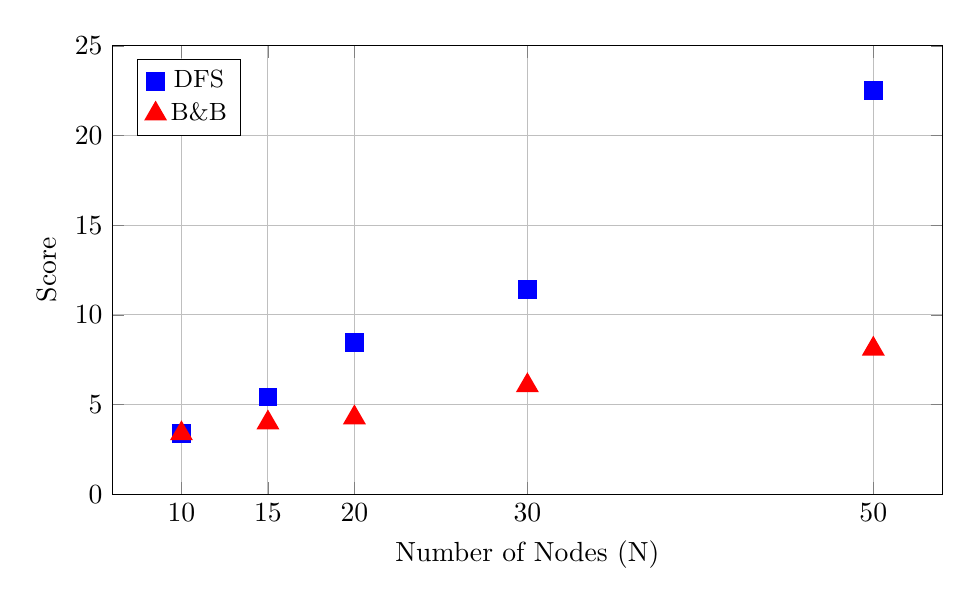
\begin{tikzpicture}
        \begin{axis}[
            width=\textwidth,
            height=0.6\textwidth,
            xlabel={Number of Nodes (N)},
            ylabel={Score},
            legend pos=north west,
            grid=major,
            xtick={10, 15, 20, 30, 50},
            ymin=0,
            ymax=25,
            legend style={font=\small}
        ]
            % DFS data
            \addplot[
                only marks,
                color=blue,
                mark=square*,
                mark size=3pt,
                thick
            ] coordinates {
                (10, 3.376)
                (15, 5.419)
                (20, 8.455)
                (30, 11.421)
                (50, 22.530)
            };
            \addlegendentry{DFS}

            % B&B data
            \addplot[
                only marks,
                color=red,
                mark=triangle*,
                mark size=4pt,
                thick
            ] coordinates {
                (10, 3.376)
                (15, 3.980)
                (20, 4.265)
                (30, 6.056)
                (50, 8.095)
            };
            \addlegendentry{B\&B}
        \end{axis}
    \end{tikzpicture}
    \caption{Comparison of DFS and Branch-and-Bound (B\&B) scores for different graph sizes.}
    \label{fig:dfs_vs_bb}
\end{figure}

Although DFS and B\&B are both able to find the optimal path, B\&B is able to find shorter paths
in a much shorter time frame. Figure \ref{fig:dfs_vs_bb} shows a comparison between the two algorithms
on the same graph sizes. 



\end{document}